\section{Introduction}
\label{intro}
The vast amount of information available in the Internet calls for \emph{personalization} schemes~\cite{bonett2001personalization}, such as \emph{recommenders}, that aid the users in their web navigation activities. Recommenders seek to suggest \emph{relevant} items to users based on their interests, by typically relying on \emph{Collaborative Filtering} (CF) algorithms~\cite{resnick1994grouplens} to leverage similarities between users. Such similarities are computed using the past rating histories of users. The axiom here is that  \emph{if Alice and Bob have liked the same items in the past, they are likely to be interested in the same items in the future}. 


\begin{figure}
\begin{center}
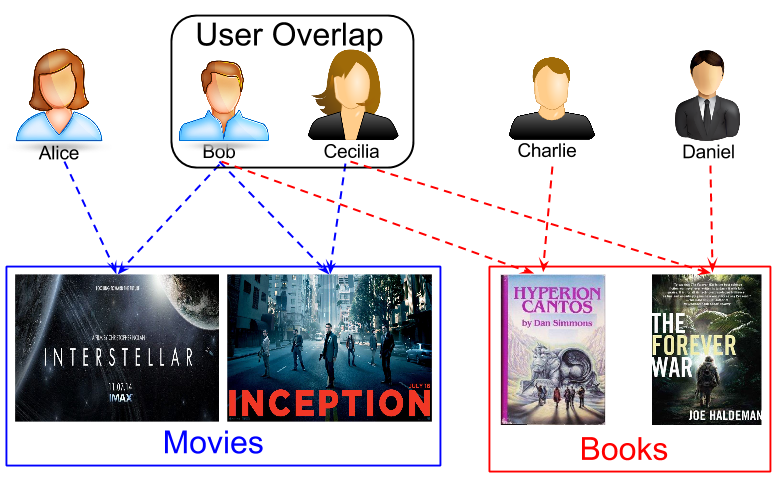
\includegraphics[height=1.7in,width=2.8in]{figures/Overlap.png}
\vspace{-4mm}
\caption{{\bf User overlap (Bob, Cecilia) with heterogeneous personalization.}}
\label{fig:overlap}
\end{center}
\end{figure}

\subsection{Motivation}


However, although widely used today, recommenders are mainly applied in a \emph{homogeneous} sense. Movie recommenders like IMDb or Netflix, news recommenders  like Google News or Yahoo News, as well as music recommenders  like Last.fm and Spotify, each focuses on a specific domain. In short, you will be recommended books if you rated books, and you will be recommended movies if you rated movies. Given the growing multiplicity of web applications, as well as  the amount of information available in the Internet, homogeneity is a major limitation. In short, with most state-of-the-art recommenders, Alice who just joined a book-oriented web application, and never rated any book before, cannot be recommended any relevant book, even if she has been rating many movies and news.

We argue that the next level to personalization is \emph{heterogeneity}, namely \emph{personalization across multiple domains}~\cite{cremonesi2011cross}. Heterogeneous preferences on the web, i.e., preferences from multiple domains, can be leveraged to improve personalization, not only for users who are new to a given domain (\emph{cold-start} situation), but also when the data is \emph{sparse}~\cite{adomavicius2005toward} (e.g, very few ratings per user). In a heterogeneous personalization scheme, if a user, say Alice, liked \emph{Interstellar}, then the system could recommend her books such as \emph{The Forever War} by Joe Haldeman. The intuition is expressed in the scenario depicted in Figure \ref{fig:overlap} where five users rated \emph{at most} one book. First, we make the following observations.
\begin{enumerate}[label=\textnormal{(\arabic*)}]
\item Alice and Bob are like-minded as both like \emph{Interstellar}\label{itm:1}.
\item Bob and Cecilia are like-minded as both like \emph{Inception}\label{itm:2}.
\item Alice and Cecilia have no common interests\label{itm:3}.
\item Alice and Cecilia are only related through Bob\label{itm:4}.
\end{enumerate}

Based on the observations \ref{itm:1}, \ref{itm:2} and \ref{itm:4}, \emph{The Forever War} could be recommended to Alice. Note that if we consider both domains as a single aggregated domain, this heterogeneous recommendation would be less likely due to the observation \ref{itm:3}.

 Heterogeneous personalization improves the quality of recommendation but it also raises several privacy concerns. For example, the new connection between Alice and Cecilia provides the opportunity for a curious user, say Alice, to discover the people (like Bob or Cecilia) who form a bridge between these two domains. She can actually probe to determine the item(s) that allows her to get this recommendation. The probing is done by masquerading as another user and incrementally rating items until the recommendation is made. By itself, her knowledge of such information poses no risk, but when used in conjunction with other information it fills a gap in knowledge that could be key to identifying the other user(s). This is similar to the privacy risk inherent in allowing statistical database queries where it is possible to make inferences from combinations of queries. Such privacy risks are amplified when the domains are owned by different companies (like IMDb for movies and Goodreads for books) which could lead to serious privacy violations.

%{\color{red} ADD MOTIVATION ABOUT PRIVACY COMPANY-BASED VS ACROSS COMPANIES}


\subsection{Challenges}

Building a simple heterogeneous recommender is straightforward by integrating ratings from both domains as a single domain. 
%Some existing work aims to address this heterogeneity problem by integrating ratings from both domains as a single domain~\cite{berkovsky2007distributed,winoto2008if, berkovsky2007cross}.
Following the aforementioned intuition (observation \ref{itm:3}), existing homogeneous personalization schemes~\cite{schafer2007collaborative, resnick1994grouplens, sarwar2001item}, if applied as such over these aggregated ratings, lead to substandard recommendation quality due to decrease in overall \emph{rating density}\footnote{Rating density is defined as the fraction of collected ratings over all the possible ratings.} as shown in Table~\ref{tab:density}. Hence, building an \emph{efficient} heterogeneous recommender is not trivial. Furthermore, making it privacy-aware is even more challenging as we discuss below.


\begin{table}[h!]
\centering
\vspace{-2mm}
\begin{tabular}{|c|c|c|c|} 
 \hline
 Books & Movies & Books+Movies\\ [0.5ex] 
 \hline
 0.0204 \% & 0.0569 \% & {\bf 0.0147 \%} \\ [1ex] 
 \hline
\end{tabular}
\caption{Densities for two domains in Amazon~\cite{mcauley2013hidden}.}
\vspace{-3mm}
\label{tab:density}
\end{table}

%Simple heterogeneous heuristics, like importing nearest neighbors from remote domains~\cite{berkovsky2007cross}, indeed improve the quality of the recommendation over homogeneous approaches, but only to a limited extent, as we show in this paper.
 %Existing homogeneous personalization schemes~\cite{schafer2007collaborative, resnick1994grouplens, sarwar2001item}, if applied as such in a heterogeneous setting, lead to substandard recommendation quality~\cite{berkovsky2007cross}. 
% cannot be applied as such in a heterogeneous sense. Berkovsky et al. empirically showed that traditional collaborative filtering algorithms are not effective~\cite{berkovsky2007cross}
%Simple heterogeneous heuristics, like importing nearest neighbors from remote domains~\cite{berkovsky2007cross}, indeed improve the quality of the recommendation over homogeneous approaches, but only to a limited extent, as we show in this paper. % are also not effective. 
% In turn, these schemes themselves are not very effective as we show in the paper.
% Heterogeneity raises several technical challenges. 
% These challenges, explained using a graph-based collaborative filtering model, are as follows.
% \subsubsection*{Similarity} 
% The first technical challenge is the \emph{similarity} computation of items, 

\noindent{\bf Similarity.} Given some user overlap across domains, a major technical challenge is to compute the \emph{similarity} between users in different domains. One might consider a graph-based similarity computation~\cite{cremonesi2011cross} where the vertices represent the items and each edge $e_{ij}$ is associated with a weight $s_{ij}$, representing the similarity between items $i$ and $j$. A \emph{path} is a sequence of adjacent vertices connected by edges in this graph. Although at first glance appealing, such an approach however ignores two factors crucial to collaborative filtering: \emph{significance weighting}~\cite{herlocker1999algorithmic} and \emph{path length}~\cite{ramakrishnan2001privacy}. Significance weighting for an item-pair ($i$,$j$) reflects the importance of the number of users who either like both items or dislike both. For equal similarities, item-pairs with higher significance weights are more crucial. Paths with shorter length provide better recommendations due to the stronger ties between item-pairs on a path~\cite{ramakrishnan2001privacy}. Homogeneous similarities have been improved based on the notion of significance weighting~\cite{herlocker1999algorithmic} as well as path length~\cite{ramakrishnan2001privacy,sun2011pathsim}. However, both factors have not been considered jointly which is crucial for accurate similarity computations in heterogeneous recommenders due to the decrease in rating density (as we show in \autoref{Sim}).

% Some recommenders have been designed with heterogeneity in mind, but as we will discuss briefly here and in more details in related work, they either make strong assumptions about the items~\cite{shi2011tags}, or do not leverage the entire information available across domains~\cite{berkovsky2007cross}. 
%As we will explain in the related work section, some recommenders that target heterogeneity assume  \emph{tagged}\footnote{A \emph{tag} is a metadata used to describe an object (e.g. Hashtags in Twitter).} items~\cite{szomszor2008correlating,szomszor2008semantic,shi2011tags}: they require a priori tagging of the items before their usage to enable the similarity computation, which is sometimes impractical due to the need of auxiliary tag-related information. Other recommenders are  \emph{knowledge-based}~\cite{li2009can} in the sense that they establish a bridge between two domains at a cluster-level
%of user-item rating patterns in order to transfer knowledge across domains\footnote{Cremonesi et al. showed that this \emph{codebook} approach does not really help heterogeneous recommendations~\cite{cremonesi2014cross}.}. Some recommenders are indeed  \emph{item-based} collaborative schemes, and do not make any assumptions on the items, but they typically consider only single and fixed-length paths between these items~\cite{cremonesi2011cross}, limiting significantly the capability of the heterogeneous recommender. 


% \subsubsection*{Scalability} 
\noindent{\bf Scalability.} Another technical challenge underlying the development of an effective heterogeneous recommender is \emph{scalability}. Assuming $m$ items in the recommender database, the time-complexity for a naive graph-based model is $O(m^2)$: this rapidly becomes a bottleneck with millions of items. For heterogeneous recommenders, the number of computations increases many-fold leading to higher computation time compared to homogeneous recommenders. %Hence, a heterogeneous recommender should support scalability for a real-world deployment.

% \subsubsection*{Privacy} 
\noindent{\bf Privacy.} As we pointed out before, \emph{privacy} is also another technical challenge for heterogeneous personalization. The advent of \emph{heterogeneous} applications increases the risk of leaking information about users. With heterogeneous applications potentially involving multiple companies, privacy is crucial: \emph{user profile should not be revealed in clear}. In addition, privacy-preserving mechanisms to prevent curious users from making inferences about someone else's input based on their recommendations are needed. The situation is even more severe with \emph{straddlers} (like Bob and Cecilia in Figure~\ref{fig:overlap}), users who connect multiple domains. Ramakrishnan et al. showed that such straddlers are at a privacy risk and information about their preference, towards items, could be used in conjunction with other data sources to uncover identities and reveal personal details~\cite{ramakrishnan2001privacy}. %Hence, privacy preservation is of prime essence in a heterogeneous recommender.



\subsection{Contributions}
In this paper, we present a recommender which we call 
% RG: we present a recommender; not an architecture
 \crossrec: \textcolor{magenta}{\texttt{\bf Cross}}-do\textcolor{magenta}{\texttt{\bf ma}}in \textcolor{magenta}{\texttt{\bf p}}ersonalization system.
In \crossrec, we fully leverage the overlap among users across multiple domains, as depicted in Figure~\ref{fig:overlap}. This overlap is often derived from profiles maintained by users across various web applications along with interconnecting mechanisms for cross-system interoperability~\cite{carmagnola2011user} and cross-system user identification~\cite{carmagnola2009user}. 
At the heart of \crossrec lie several schemes. 

\begin{itemize}
\item \crossrec leverages a novel similarity metric, \graphsim, which computes a meta path-based transitive closure of item-item similarities across several domains while supporting the two crucial factors: \emph{significance weighting} and \emph{path length}. \graphsim is leveraged to compute artificial profiles of users even in domains where they have \emph{no} or \emph{very little} activity yet. 

\item We capture these artificial profiles through our notion of \emph{AlterEgo}.  \crossrec generates an \emph{AlterEgo} profile (of Alice) in the target domain leveraging an item-to-item mapping from a source domain (e.g., movies) to a target domain (e.g., books). We present a private technique (in \crossrec) as well as a non-private one (in \npcrossrec) for generating the AlterEgo profiles. Note that \npcrossrec illustrates the effectiveness of \graphsim and \emph{AlterEgo} profiles for heterogeneous recommendations without the additional privacy overhead and could be used for applications with heterogeneous intra-company services like \emph{Amazon} or \emph{Google Play}. We demonstrate the flexibility of \crossrec to integrate auxiliary recommendation features in the target domain by incorporating a differentially private approach inspired by Zhu et al.~\cite{zhu2013differential,zhu2014effective} to provide the final recommendations. \npcrossrec significantly outperforms the quality of alternative heterogeneous systems~\cite{baltrunas2009context,lemire2005slope,berkovsky2007cross,sarwar2001item, cremonesi2011cross} whereas \crossrec (even with the additional privacy overhead) still provides better quality compared to the non-private alternatives.

%To illustrate the effectiveness of \graphsim and \emph{AlterEgo} for heterogeneous recommendations without any privacy overhead, we implemented a non-private variant of \crossrec denoted by \npcrossrec. We show that the quality of recommendations provided by \npcrossrec, leveraging the AlterEgo profiles in the target domain, significantly outperforms the quality of alternative heterogeneous systems~\cite{baltrunas2009context,lemire2005slope,berkovsky2007cross,sarwar2001item, cremonesi2011cross}. Furthermore, \crossrec, with the additional privacy overhead, still provides slightly better quality compared to the non-private alternatives. We demonstrate that \crossrec can provide better recommendations during cold-start as well as when the sparsity of the dataset is high. 

\item We implement \crossrec on top of Apache Spark to achieve scalability and fault tolerance. We show that \crossrec scales almost linearly with an increasing number of machines (a major requirement for the deployment of a recommender in a practical environment). %\framework scales up by 5.2$\times$ on a cluster size of 15. 

\item We deployed an online recommendation platform, leveraging \graphsim on a database of around 660K items, to recommend books and movies to users based on their \emph{searched} product at\footnote{Currently, we support only Chrome, Safari and Firefox browsers.}: \begin{center}\vspace{-2mm} \url{http://x-map.work/} \vspace{-3mm}\end{center}
We observe that it can recommend books like \emph{The Da Vinci Code} when the search query is \emph{Angels \& Demons} (2009) movie. 
\end{itemize}

\subsection{Roadmap}

The rest of the paper is structured as follows. We provide some preliminaries on collaborative filtering before formulating the heterogeneity problem for recommenders in \autoref{background}. Next, we introduce our \graphsim metric in \autoref{Sim}. We distinguish the private recommendation scheme underlying \crossrec from the non-private one (\npcrossrec) in \autoref{Recommendation}. Then, we present our scalable implementation of \crossrec in \autoref{Implementation}. We present our experimental results in \autoref{Evaluation} and then review the related work in \autoref{RelWorks}. Finally, we conclude our paper in \autoref{Conclusion}. {\color{red}For space limitations, we defer the detailed proofs to our companion technical report~\cite{} for interested readers.}
